\documentclass[11pt,a4paper]{article}
\usepackage[T1]{fontenc}
\usepackage[utf8]{inputenc}
\usepackage{lmodern}
\usepackage{textcomp}
\usepackage[left=1.8cm,right=1.8cm,top=2.3cm,bottom=2.2cm,headheight=14pt,headsep=8pt]{geometry}
\usepackage{multicol}
\usepackage{xcolor}
\usepackage{fancyhdr}
\usepackage{graphicx}
\usepackage{array}
\usepackage{amsmath,amssymb}
\usepackage{setspace}
\usepackage{longtable}
\graphicspath{{../}}
\definecolor{ygreen}{RGB}{46,139,87}
\renewcommand{\normalsize}{\fontsize{10.9}{13.4}\selectfont}
\renewcommand{\familydefault}{\rmdefault}
\setlength{\parindent}{0pt}
\setlength{\columnsep}{0.8cm}
\setlength{\columnseprule}{0.4pt}
\setlength{\multicolsep}{3pt plus 1pt minus 1pt}
\renewcommand{\textsubscript}[1]{\ensuremath{_{\text{\fontsize{8}{8}\selectfont #1}}}}
\renewcommand{\textsuperscript}[1]{\ensuremath{^{\text{\fontsize{8}{8}\selectfont #1}}}}
\newcommand{\diqqat}[1]{\par\smallskip\noindent\textbf{Diqqat!} #1\par\medskip}
\newcommand{\javob}{\par\smallskip\noindent\textbf{Javob:} \rule[-2pt]{7.5cm}{0.4pt}\par\smallskip\noindent\textbf{Diqqat!} Javobingizni javoblar varaqasiga ko`chirib yozing.\par\medskip}
\pagestyle{fancy}
\fancyhf{}
\renewcommand{\headrulewidth}{0.4pt}
\fancyhead[L]{\textit{Milliy sertifikat 2026. Kimyo}}
\fancyhead[R]{10-variant}
\fancyfoot[L]{\fontsize{8}{9}\selectfont \textcopyright{} Colba maktabi, 2026}
\fancyfoot[C]{\thepage}
\fancypagestyle{first}{\fancyhf{}\renewcommand{\headrulewidth}{0pt}\fancyfoot[L]{\fontsize{8}{9}\selectfont \textcopyright{} Colba maktabi, 2026}\fancyfoot[C]{\thepage}}
\begin{document}
\normalsize
\thispagestyle{first}
\noindent\fcolorbox{ygreen}{white}{\parbox{\dimexpr\linewidth-2\fboxsep-2\fboxrule\relax}{%
\textbf{\fontsize{13}{15}\selectfont Nazorat testi}\ \textit{\fontsize{10}{12}\selectfont $\cdot$ Aralash test $\cdot$ 10-variant}\hfill
\begin{tabular}[t]{@{}r@{}}\textit{Milliy sertifikat 2026. Kimyo}\\ \textbf{\textit{\fontsize{8}{9}\selectfont Vaqt:}} \textit{\fontsize{10}{12}\selectfont 180 daqiqa}\end{tabular}}}
\par\medskip
\noindent\textit{Davriy jadvaldan foydalanish mumkin.}
\par\medskip
\begin{multicols}{2}
\noindent\textbf{1.} CO + H\textsubscript{2}O $\rightleftarrows$ CO\textsubscript{2} + H\textsubscript{2} reaksiyasi 4 l hajmli idishda o`tkazildi. Ma'lumotlar jadvalda berilgan:
\begin{center}
\renewcommand{\arraystretch}{1.15}
\begin{tabular}{|c|c|c|c|}\hline
\textbf{Modda} & \textbf{CO} & \textbf{H\textsubscript{2}O} & \textbf{CO\textsubscript{2}} \\ \hline
Boshlang`ich, mol & 6 & 3 & 0 \\ \hline
Muvozanatda, mol & --- & --- & 2 \\ \hline
\end{tabular}
\end{center}
Muvozanat \textbf{konstantasini (K) hisoblang.}

\noindent A)~\textsl{2} \hfill B)~\textsl{1} \hfill C)~\textsl{0,5} \hfill D)~\textsl{4}\par
\vspace{4pt}
\noindent\textbf{2.} Rasmda neytral atom elektron qavatlarining orbital diagrammasi (kataklar -- orbitallar, o`qlar -- elektronlar) berilgan.
\begin{center}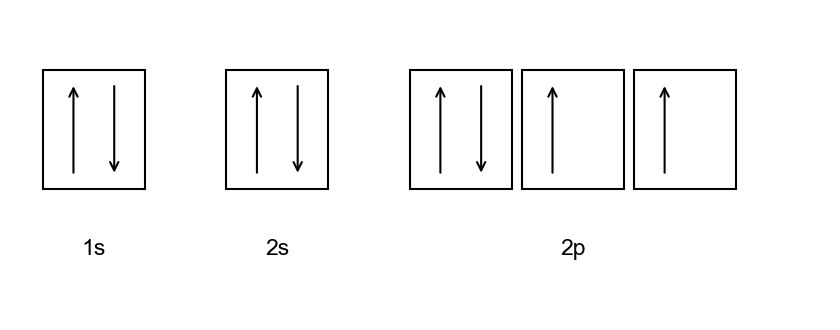
\includegraphics[width=0.86\linewidth]{rasmlar/gen/or_128790.png}\end{center}
Diagramma qaysi element atomiga tegishli?

\noindent A)~\textsl{ftor} \hfill B)~\textsl{neon} \hfill C)~\textsl{kislorod} \hfill D)~\textsl{uglerod}\par
\vspace{4pt}
\noindent\textbf{3.} Faqat oksidlovchi bo`la oladigan \textbf{ionlarni aniqlang}: 1) Zn\textsuperscript{2+}; 2) Fe\textsuperscript{2+}; 3) Cl\textsuperscript{$-$}; 4) Fe\textsuperscript{3+}

\noindent A)~\textsl{1, 2} \hfill B)~\textsl{2, 4} \hfill C)~\textsl{1} \hfill D)~\textsl{1, 3}\par
\vspace{4pt}
\noindent\textbf{4.} Massa soni 226 va zaryadi 88 bo`lgan yadro massa soni 206, zaryadi 82 bo`lgan yadroga aylanishida nechta $\alpha$- va $\beta$\textsuperscript{$-$}-zarra chiqaradi?

\noindent A)~\textsl{6$\alpha$ va 4$\beta$} \hfill B)~\textsl{5$\alpha$ va 4$\beta$} \hfill C)~\textsl{5$\alpha$ va 6$\beta$} \hfill D)~\textsl{4$\alpha$ va 5$\beta$}\par
\vspace{4pt}
\noindent\textbf{5.} 25 ml HCl eritmasi 0,05 mol/l li NaOH eritmasi bilan titrlandi. Titrlash egri chizig`i grafikda berilgan (ekvivalent nuqta 25 ml da).
\begin{center}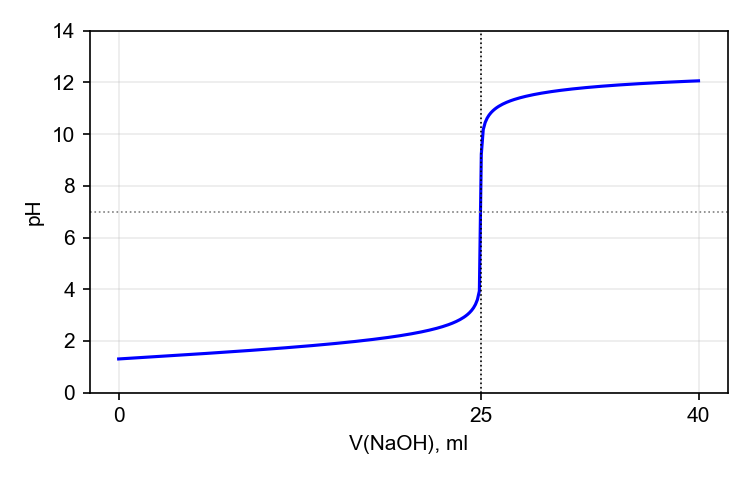
\includegraphics[width=0.86\linewidth]{rasmlar/gen/ti_v10_0.png}\end{center}
Grafikning boshlang`ich nuqtasi (\textit{V} = 0) pH ining qiymatiga mos keluvchi HCl eritmasidagi H\textsuperscript{+} \textbf{konsentratsiyasini (mol/l) toping.}

\noindent A)~\textsl{0,5} \hfill B)~\textsl{0,005} \hfill C)~\textsl{0,05} \hfill D)~\textsl{0,1}\par
\vspace{4pt}
\noindent\textbf{6.} 20 l NO va 30 l O\textsubscript{2} aralashmasi 2NO + O\textsubscript{2} $\to$ 2NO\textsubscript{2} tenglama bo`yicha to`liq reaksiyaga kirishdi (barcha gazlar bir xil sharoitda o`lchandi). Aralashma hajmi necha litrga o`zgargan (modul bo`yicha)?

\noindent A)~\textsl{10} \hfill B)~\textsl{50} \hfill C)~\textsl{40} \hfill D)~\textsl{20}\par
\vspace{4pt}
\noindent\textbf{7.} 2NO + O\textsubscript{2} $\rightleftarrows$ 2NO\textsubscript{2} reaksiyada muvozanat holatida [NO] = 0,5, [O\textsubscript{2}] = 2, [NO\textsubscript{2}] = 4 mol/l. Muvozanat \textbf{konstantasini (K) hisoblang.}

\noindent A)~\textsl{64} \hfill B)~\textsl{16} \hfill C)~\textsl{4} \hfill D)~\textsl{32}\par
\vspace{4pt}
\noindent\textbf{8.} 11,2 g Fe va 9,6 g S aralashtirilib, reaksiya o`tkazildi (Fe + S $\to$ FeS). Hosil bo`lgan FeS \textbf{massasini (g) aniqlang.}

\noindent A)~\textsl{26,4} \hfill B)~\textsl{35,2} \hfill C)~\textsl{8,8} \hfill D)~\textsl{17,6}\par
\vspace{4pt}
\noindent\textbf{9.} Quyidagi jadvalda Na\textsubscript{2}CO\textsubscript{3} tuzining eritmalari keltirilgan:
\begin{center}
\renewcommand{\arraystretch}{1.15}
\begin{tabular}{|c|c|c|}\hline
\textbf{No.} & \textbf{m(eritma), g} & \textbf{$\omega$, \%} \\ \hline
I & 150 & 12 \\ \hline
II & 100 & 30 \\ \hline
\end{tabular}
\end{center}
Eritmalar aralashtirildi. Oxirgi eritmadagi tuzning massa \textbf{ulushini (\%) toping.}

\noindent A)~\textsl{21} \hfill B)~\textsl{42} \hfill C)~\textsl{22,8} \hfill D)~\textsl{19,2}\par
\vspace{4pt}
\noindent\textbf{10.} Tabiiy elementning ikki izotopi: \textsuperscript{63}Cu (70\%) va \textsuperscript{65}Cu (30\%). Elementning o`rtacha nisbiy atom \textbf{massasini aniqlang.}

\noindent A)~\textsl{64} \hfill B)~\textsl{64,4} \hfill C)~\textsl{63,6} \hfill D)~\textsl{63}\par
\vspace{4pt}
\noindent\textbf{11.} Quyidagi zarrachalardan qaysilari neon atomi bilan izoelektron? 1) N\textsuperscript{3$-$}; 2) Al\textsuperscript{3+}; 3) Cl\textsuperscript{$-$}; 4) Ca\textsuperscript{2+}

\noindent A)~\textsl{2, 3, 4} \hfill B)~\textsl{1, 2} \hfill C)~\textsl{2, 3} \hfill D)~\textsl{1, 3}\par
\vspace{4pt}
\noindent\textbf{12.} 2 mol Ba(OH)\textsubscript{2} va 2 mol HNO\textsubscript{3} suvda eritilib, eritma hajmi 2 l ga yetkazildi. Eritmadagi barcha ionlarning umumiy molyar \textbf{konsentratsiyasini (mol/l) aniqlang} (kuchli elektrolitlar to`liq dissotsilanadi).

\noindent A)~\textsl{2} \hfill B)~\textsl{10} \hfill C)~\textsl{2,5} \hfill D)~\textsl{5}\par
\vspace{4pt}
\noindent\textbf{13.} Na\textsubscript{2}SO\textsubscript{4}$\cdot$10H\textsubscript{2}O kristallogidratida kristallizatsion suvning massa \textbf{ulushini (\%) aniqlang.}

\noindent A)~\textsl{55,9} \hfill B)~\textsl{44,1} \hfill C)~\textsl{28} \hfill D)~\textsl{126,8}\par
\vspace{4pt}
\noindent\textbf{14.} Quyidagi tuzlardan qaysilari asosli tuz? 1) K\textsubscript{2}SO\textsubscript{4}; 2) (CuOH)\textsubscript{2}CO\textsubscript{3}; 3) CaCO\textsubscript{3}; 4) KAl(SO\textsubscript{4})\textsubscript{2}

\noindent A)~\textsl{2, 4} \hfill B)~\textsl{2} \hfill C)~\textsl{2, 3} \hfill D)~\textsl{4}\par
\vspace{4pt}
\noindent\textbf{15.} 2Al + 3CuCl\textsubscript{2} $\to$ 2AlCl\textsubscript{3} + 3Cu reaksiyasida 6,75 g Al ishtirok etdi. Cu \textbf{miqdorini (mol) toping.}

\noindent A)~\textsl{0,17} \hfill B)~\textsl{0,75} \hfill C)~\textsl{0,19} \hfill D)~\textsl{0,38}\par
\vspace{4pt}
\noindent\textbf{16.} Nodir gazlar haqida qaysi fikrlar to`g`ri? 1) Geliy eng yengil inert gaz; 2) Neon reklama naylarida ishlatiladi; 3) Nodir gazlar odatiy sharoitda ko`p atomli molekulalar hosil qiladi; 4) Argon havoning hajmi bo`yicha eng ko`p uchraydigan inert gazi

\noindent A)~\textsl{1, 2} \hfill B)~\textsl{1, 2, 4} \hfill C)~\textsl{1, 2, 3} \hfill D)~\textsl{3, 4}\par
\vspace{4pt}
\noindent\textbf{17.} 47 g Cu(NO\textsubscript{3})\textsubscript{2} to`liq parchalanguncha qizdirildi. Qattiq qoldiq \textbf{massasini (g) aniqlang.}

\noindent A)~\textsl{47} \hfill B)~\textsl{40} \hfill C)~\textsl{10} \hfill D)~\textsl{20}\par
\vspace{4pt}
\noindent\textbf{18.} 60 g FeS\textsubscript{2} yondirilib, hosil bo`lgan SO\textsubscript{2} dan H\textsubscript{2}SO\textsubscript{4} olindi (jami unum 80\%). Sulfat kislota \textbf{massasini (g) aniqlang.}

\noindent A)~\textsl{78,4} \hfill B)~\textsl{49} \hfill C)~\textsl{156,8} \hfill D)~\textsl{98}\par
\vspace{4pt}
\noindent\textbf{19.} Zn(NO\textsubscript{3})\textsubscript{2} qizdirilganda qanday moddalar hosil bo`ladi?

\noindent\begin{tabular}{@{}p{0.47\linewidth}@{}p{0.47\linewidth}@{}}
A)~\textsl{Ag, NO\textsubscript{2} va O\textsubscript{2}} & B)~\textsl{ZnO, NO\textsubscript{2} va O\textsubscript{2}} \\
C)~\textsl{NaNO\textsubscript{2} va O\textsubscript{2}} & D)~\textsl{KNO\textsubscript{2} va O\textsubscript{2}} \\
\end{tabular}\par
\vspace{4pt}
\noindent\textbf{20.} 25,25 g CH\textsubscript{3}Cl dan quyidagi ikki bosqichda HCl olinadi: 1) 2CH\textsubscript{3}Cl + 2Na $\to$ C\textsubscript{2}H\textsubscript{6} + 2NaCl (unum 90\%); 2) C\textsubscript{2}H\textsubscript{6} + Cl\textsubscript{2} $\to$ C\textsubscript{2}H\textsubscript{5}Cl + HCl (unum 50\%). Oxirgi mahsulot HCl ning \textbf{hajmini (l, n.sh.) toping.}

\noindent A)~\textsl{2,8} \hfill B)~\textsl{5,04} \hfill C)~\textsl{5,6} \hfill D)~\textsl{2,52}\par
\vspace{4pt}
\noindent\textbf{21.} CH\textsubscript{2}=CH--CH\textsubscript{2}--CH\textsubscript{3} birikmaning sistematik nomi qaysi qatorda to`g`ri keltirilgan?

\noindent A)~\textsl{buten-1} \hfill B)~\textsl{buten-2} \hfill C)~\textsl{1-butin} \hfill D)~\textsl{butan}\par
\vspace{4pt}
\noindent\textbf{22.} Arenlar, neft va tabiiy gaz haqida qaysi fikrlar to`g`ri? 1) Benzol bromli suvni rangsizlantirmaydi; 2) Tabiiy gazning asosiy qismi propan; 3) Neft fraksiyalaridan gazolin 150 \textdegree{}C gacha haydaladi; 4) Benzoldan nitrobenzol nitrolash bilan olinadi

\noindent A)~\textsl{3, 4} \hfill B)~\textsl{1, 2} \hfill C)~\textsl{1, 3, 4} \hfill D)~\textsl{2, 3, 4}\par
\vspace{4pt}
\noindent\textbf{23.} CH\textsubscript{3}CHO + Ag\textsubscript{2}O (NH\textsubscript{3}) reaksiyasi natijasida qaysi organik modda hosil bo`ladi?

\noindent\begin{tabular}{@{}p{0.47\linewidth}@{}p{0.47\linewidth}@{}}
A)~\textsl{etilatsetat} & B)~\textsl{etanol} \\
C)~\textsl{sirka kislota} & D)~\textsl{metan} \\
\end{tabular}\par
\vspace{4pt}
\noindent\textbf{24.} Aldegid va ketonlar haqida qaysi fikrlar to`g`ri? 1) Formaldegid gaz holatda, suvda yaxshi eriydi; 2) Ketonlar kuchsiz oksidlovchilar bilan oksidlanmaydi; 3) Aldegidlar qaytarilganda ikkilamchi spirt hosil bo`ladi; 4) Sirka aldegid Kucherov reaksiyasi bilan olinadi

\noindent A)~\textsl{1, 2, 4} \hfill B)~\textsl{1, 4} \hfill C)~\textsl{1, 2} \hfill D)~\textsl{2, 3}\par
\vspace{4pt}
\noindent\textbf{25.} 2HCOOH + Mg $\to$ (HCOO)\textsubscript{2}Mg + H\textsubscript{2} jarayoni uchun 18,4 g HCOOH olingan. H\textsubscript{2} \textbf{hajmini (l, n.sh.) aniqlang.}

\noindent A)~\textsl{4,48} \hfill B)~\textsl{17,92} \hfill C)~\textsl{8,96} \hfill D)~\textsl{2,24}\par
\vspace{4pt}
\noindent\textbf{26.} Murakkab efirlar va yog`lar haqida qaysi fikrlar to`g`ri? 1) Efirlanish reaksiyasi qaytmas; 2) Etilatsetat efir hidli suyuqlik; 3) Suyuq yog`larni gidrogenlab qattiq yog` olinadi; 4) Suyuq yog`lar to`yinmagan kislotalardan hosil bo`lgan

\noindent A)~\textsl{2, 3, 4} \hfill B)~\textsl{1, 2} \hfill C)~\textsl{1, 4} \hfill D)~\textsl{2, 4}\par
\vspace{4pt}
\noindent\textbf{27.} Reaksiya tenglamasi: C\textsubscript{12}H\textsubscript{22}O\textsubscript{11} + H\textsubscript{2}O $\to$ 2C\textsubscript{6}H\textsubscript{12}O\textsubscript{6}. Reaksiyaga 684 g C\textsubscript{12}H\textsubscript{22}O\textsubscript{11} kirishdi. C\textsubscript{6}H\textsubscript{12}O\textsubscript{6} \textbf{massasini (g) hisoblang.}

\noindent A)~\textsl{180} \hfill B)~\textsl{720} \hfill C)~\textsl{1440} \hfill D)~\textsl{360}\par
\vspace{4pt}
\noindent\textbf{28.} 26,7 g alanin HCl bilan reaksiyaga kirishganda hosil bo`lgan tuz \textbf{massasini (g) aniqlang.}

\noindent A)~\textsl{26,7} \hfill B)~\textsl{37,65} \hfill C)~\textsl{10,95} \hfill D)~\textsl{75,3}\par
\vspace{4pt}
\noindent\textbf{29.} C\textsubscript{2}H\textsubscript{4} + Cl\textsubscript{2} $\to$ C\textsubscript{2}H\textsubscript{4}Cl\textsubscript{2} reaksiyasida 4,48 l (n.sh.) Cl\textsubscript{2} ishtirok etdi. C\textsubscript{2}H\textsubscript{4}Cl\textsubscript{2} \textbf{massasini (g) toping.}

\noindent A)~\textsl{19,8} \hfill B)~\textsl{39,6} \hfill C)~\textsl{9,9} \hfill D)~\textsl{29,7}\par
\vspace{4pt}
\noindent\textbf{30.} Eritmaga NaOH (qizdirilganda) qo`shilganda o`tkir hidli gaz (NH\textsubscript{3}) kuzatildi. Eritmada qaysi ion bor?

\noindent A)~\textsl{Ba\textsuperscript{2+}} \hfill B)~\textsl{SO\textsubscript{4}\textsuperscript{2$-$}} \hfill C)~\textsl{NH\textsubscript{4}\textsuperscript{+}} \hfill D)~\textsl{I\textsuperscript{$-$}}\par
\vspace{4pt}
\noindent\textbf{31.} Metiloranj indikatori ishqoriy muhitda qanday rang beradi?
\noindent A)~\textsl{ko`k}\par
\noindent B)~\textsl{malina rangga kiradi (pushti)}\par
\noindent C)~\textsl{rangsiz}\par
\noindent D)~\textsl{sariq}\par
\vspace{4pt}
\noindent\textbf{32.} Rasmdagi asbobda olingan ammiak qanday yig`iladi?
\begin{center}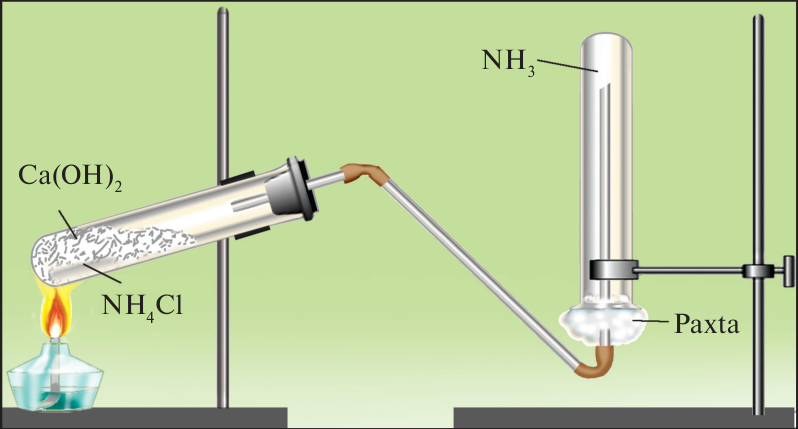
\includegraphics[width=0.86\linewidth]{rasmlar/darslik/d_nh3_lab.png}\end{center}
\noindent A)~\textsl{og`zi yuqoriga qaratilgan idishda}\par
\noindent B)~\textsl{suvni siqib chiqarish usulida}\par
\noindent C)~\textsl{og`zi pastga qaratilgan probirkada, havoni siqib chiqarish usulida}\par
\noindent D)~\textsl{yig`ib bo`lmaydi   ---}\par
\vspace{4pt}
\end{multicols}
\medskip
\noindent\setlength{\fboxsep}{0pt}\fbox{\begin{tabular}{p{0.74\linewidth}|p{0.2\linewidth}}
\parbox[t]{0.72\linewidth}{\vspace{3pt}\textbf{Topshiriqlar (33--35) va javob variant (A--F)larini o`zaro to`g`ri moslashtiring.} Sirka kislota va etanoldan iborat 16,6 g aralashmaga mo`l NaHCO\textsubscript{3} eritmasi qo`shilganda 4,48 l (n.sh.) gaz ajraldi. Xuddi shunday massadagi aralashma natriy bilan ta'sirlashganda esa 3,36 l (n.sh.) vodorod ajraldi.
\vspace{3pt}} & \parbox[t]{0.19\linewidth}{\vspace{3pt}A~\textsl{9,6}\\[3pt]
B~\textsl{6,9}\\[3pt]
C~\textsl{12}\\[3pt]
D~\textsl{4,6}\\[3pt]
E~\textsl{26,24}\\[3pt]
F~\textsl{13,12}}\\ \hline
\parbox[t]{0.72\linewidth}{\vspace{2pt}\textbf{33. Aralashmadagi sirka kislota massasini (g) aniqlang.}\vspace{2pt}} & \\ \hline
\parbox[t]{0.72\linewidth}{\vspace{2pt}\textbf{34. Aralashmadagi etanol massasini (g) aniqlang.}\vspace{2pt}} & \\ \hline
\parbox[t]{0.72\linewidth}{\vspace{2pt}\textbf{35. Aralashma to`liq neytrallanganda (faqat kislota) hosil bo`lgan natriy atsetat massasini (g) aniqlang (reaksiya unumi 80\%).}\vspace{2pt}} & 
\end{tabular}}
\par\bigskip
\noindent\textbf{36.} S + HNO\textsubscript{3} $\to$ H\textsubscript{2}SO\textsubscript{4} + NO reaksiya tenglamasini tenglang va barcha koeffitsiyentlar \textbf{yig`indisini aniqlang.}
\javob
\noindent\textbf{37.} CH\textsubscript{4} va H\textsubscript{2} dan iborat 60 ml aralashma mo`l kisloroda yondirildi (suv suyuq holatda; hajmlar bir xil sharoitda o`lchandi). Reaksiyadan so`ng gazlar hajmi 100 ml ga kamaydi. Aralashmadagi CH\textsubscript{4} \textbf{hajmini (ml) toping.}
\javob
\noindent\textbf{38.} 29,6 g Mg(NO\textsubscript{3})\textsubscript{2} to`liq parchalanguncha qizdirildi. Qattiq qoldiq \textbf{massasini (g) aniqlang.}
\javob
\noindent\textbf{39.} To`yingan bir atomli karbon kislotaning 4,6 g massasi mo`l NaHCO\textsubscript{3} eritmasi bilan reaksiyaga kirishganda 2,24 l (n.sh.) CO\textsubscript{2} ajraldi. Kislotaning molyar \textbf{massasini (g/mol) aniqlang.}
\javob
\noindent\textbf{40.} 5,2 g asetilendan Kucherov reaksiyasi bilan (80\% unum) sirka aldegid olindi. Aldegid \textbf{massasini (g) aniqlang.}
\javob
\par\bigskip\begin{center}\textbf{\fontsize{13}{15}\selectfont YOZMA ISH}\end{center}
\noindent\textbf{41.} \textbf{Topshiriqni bajarish jarayonida barcha reaksiya tenglamalarini yozing. Miqdoriy va arifmetik hisoblashlarni (unga asos bo`lgan usul yoki formulani ko`rsatgan holda) uzviy ketma-ketlikda bajaring.}\par\smallskip
HCOONa tuzining 0,01 mol/l li suvli eritmasi berilgan. HCOOH ning dissotsilanish konstantasi Ka = 1$\cdot$10\textasciicircum{}-4, K(suv) = 1$\cdot$10\textsuperscript{$-$14}.\par
\noindent 1)Tuzning gidrolizlanish reaksiyasi tenglamasini yozing va gidroliz konstantasini (Kh) hisoblang.\par
\noindent 2)Eritmadagi OH\textsuperscript{$-$} ionlarining konsentratsiyasini (mol/l) toping. pOH ni ham hisoblang.\par
\noindent 3)Eritmaning pH ini hisoblang.\par
\noindent 4)Gidrolizlanish darajasini (\%) aniqlang. Eritmadagi H\textsuperscript{+} konsentratsiyasini (mol/l) ham toping.\par
\noindent 5)Shunday eritmadan 500 ml tayyorlash uchun necha gramm HCOONa kerak? Eritma 10 marta suyultirilsa gidrolizlanish darajasi necha marta ortadi?\par
\diqqat{Mazkur topshiriq kengaytirilgan javobni talab etib, uning yechilish usuli va shu usul asosidagi barcha hisoblash amallari javoblar varaqasida aks etishi lozim.}
\noindent\textbf{42.} Quyidagi o`zgarishlar zanjirida \textit{X}, \textit{Y}, \textit{Z} noma'lum organik moddalar:\par
\[\setlength{\fboxsep}{0pt}\text{CH\textsubscript{4}}\xrightarrow{\text{Cl\textsubscript{2}, yorug`lik}}\text{\textit{X}}\xrightarrow{\text{Na}}\text{\textit{Y}}\xrightarrow{\text{Cl\textsubscript{2}, yorug`lik}}\text{\textit{Z}}\xrightarrow{\text{KOH (spirtli)}}\text{C\textsubscript{2}H\textsubscript{4}}\]
\noindent 1)CH\textsubscript{4} $\to$ \textit{X} : reaksiya tenglamasini yozing; hosil bo`lgan moddani nomlang.\par
\noindent 2)\textit{X} $\to$ \textit{Y} : reaksiya tenglamasini yozing; hosil bo`lgan moddani nomlang.\par
\noindent 3)\textit{Y} $\to$ \textit{Z} : reaksiya tenglamasini yozing; hosil bo`lgan moddani nomlang.\par
\noindent 4)\textit{Z} $\to$ C\textsubscript{2}H\textsubscript{4} : reaksiya tenglamasini yozing; hosil bo`lgan moddani nomlang.\par
\diqqat{Mazkur topshiriq kengaytirilgan javobni talab etib, uning yechilish usuli va shu usul asosidagi barcha hisoblash amallari javoblar varaqasida aks etishi lozim.}
\noindent\textbf{43.} \textbf{Topshiriqni bajarish jarayonida barcha reaksiya tenglamalarini yozing. Miqdoriy va arifmetik hisoblashlarni (unga asos bo`lgan usul yoki formulani ko`rsatgan holda) uzviy ketma-ketlikda bajaring.}\par\smallskip
Uch probirkada XCl\textsubscript{2}, YCl\textsubscript{2} va ZCl\textsubscript{2} tarkibli metall xloridlarining eritmalari bor. Har bir eritmaga reagentlar ta'sir ettirildi, kuzatuvlar jadvalda ("---" belgisi reaksiya bormasligini bildiradi, bo`sh kataklar bo`yicha ma'lumot berilmagan):\par
\begin{center}
\renewcommand{\arraystretch}{1.15}
\begin{tabular}{|c|c|c|c|}\hline
\textbf{Reagent} & \textbf{XCl\textsubscript{2}} & \textbf{YCl\textsubscript{2}} & \textbf{ZCl\textsubscript{2}} \\ \hline
H\textsubscript{2}S & qora cho`kma & --- &  \\ \hline
Na\textsubscript{2}S & qora cho`kma & qora cho`kma & oq cho`kma \\ \hline
NaOH & havorang cho`kma & och yashil cho`kma & oq cho`kma \\ \hline
Zn plastinka & qizil qoplama &  & --- \\ \hline
\end{tabular}
\end{center}
\textit{X}, \textit{Y}, \textit{Z} --- davriy sistemaning to`rtinchi davridagi metallar.\par
\noindent 1)Jadvalda kuzatilgan barcha reaksiyalarning molekulyar tenglamalarini yozing. XCl\textsubscript{2} eritmasiga tushirilgan Zn plastinkada 0,1 mol \textit{X} ajralgan bo`lsa, plastinka massasi qanchaga (g) o`zgargan?\par
\noindent 2)\textit{X}, \textit{Y}, \textit{Z} metallarni aniqlang va tuzlarning formulalarini yozing. XCl\textsubscript{2} tarkibida \textit{X} ning massa ulushi 47,4\% ekanini hisob bilan tasdiqlang.\par
\noindent 3)12,7 g YCl\textsubscript{2} eritmasiga mo`l NaOH qo`shildi, hosil bo`lgan cho`kma havoda to`liq oksidlanguncha qoldirildi. Barcha reaksiya tenglamalarini yozing va oxirgi cho`kma massasini (g) aniqlang.\par
\noindent 4)ZCl\textsubscript{2} ning 13,6 g massasi mo`l NaOH eritmasi bilan reaksiyaga kirishganda hosil bo`lgan kompleks tuz massasini (g) hisoblang (reaksiya tenglamalarini yozing).\par
\noindent 5)Hosil bo`lgan Cu(OH)\textsubscript{2} cho`kmasi (0,1 mol) qizdirilganda hosil bo`ladigan CuO massasini (g) hisoblang.\par
\diqqat{Mazkur topshiriq kengaytirilgan javobni talab etib, uning yechilish usuli va shu usul asosidagi barcha hisoblash amallari javoblar varaqasida aks etishi lozim.}
\newpage
\noindent\textbf{\fontsize{13}{15}\selectfont Nazorat testi}\ \textit{$\cdot$ 10-variant}\hfill \textbf{Javoblar kaliti}\par\smallskip\hrule\smallskip
\textit{Faqat o`qituvchi uchun.}\par\medskip
\noindent\textbf{1--32-savollar}\par\smallskip
\noindent\begin{tabular}{|c|c|c|c|c|c|c|c|c|c|c|c|c|c|c|c|}\hline
\textbf{1} & \textbf{2} & \textbf{3} & \textbf{4} & \textbf{5} & \textbf{6} & \textbf{7} & \textbf{8} & \textbf{9} & \textbf{10} & \textbf{11} & \textbf{12} & \textbf{13} & \textbf{14} & \textbf{15} & \textbf{16}\\\hline
\textsl{B} & \textsl{C} & \textsl{C} & \textsl{B} & \textsl{C} & \textsl{A} & \textsl{D} & \textsl{D} & \textsl{D} & \textsl{C} & \textsl{B} & \textsl{D} & \textsl{A} & \textsl{B} & \textsl{D} & \textsl{B}\\\hline
\textbf{17} & \textbf{18} & \textbf{19} & \textbf{20} & \textbf{21} & \textbf{22} & \textbf{23} & \textbf{24} & \textbf{25} & \textbf{26} & \textbf{27} & \textbf{28} & \textbf{29} & \textbf{30} & \textbf{31} & \textbf{32}\\\hline
\textsl{D} & \textsl{A} & \textsl{B} & \textsl{D} & \textsl{A} & \textsl{C} & \textsl{C} & \textsl{A} & \textsl{A} & \textsl{A} & \textsl{B} & \textsl{B} & \textsl{A} & \textsl{C} & \textsl{D} & \textsl{C}\\\hline
\end{tabular}\par\medskip
\noindent\textbf{33--35-savollar}\par\smallskip
\noindent\begin{tabular}{|c|c|c|}\hline \textbf{No} & \textbf{Javob} & \textbf{Qiymat}\\\hline
33 & \textsl{C} & 12\\\hline
34 & \textsl{D} & 4,6\\\hline
35 & \textsl{F} & 13,12\\\hline
\end{tabular}\par\medskip
\noindent\textbf{36--40-savollar}\par\smallskip
\noindent\begin{tabular}{|c|c|}\hline \textbf{No} & \textbf{To`g`ri javob}\\\hline
36 & 6\\\hline
37 & 20\\\hline
38 & 8\\\hline
39 & 46\\\hline
40 & 7,04\\\hline
\end{tabular}\par\medskip
\noindent\textbf{41--43-topshiriqlar: qisqa yechim}\par\smallskip
\noindent\textbf{41-topshiriq.}\par
\noindent 1) HCOONa + H\textsubscript{2}O $\rightleftarrows$ HCOOH + NaOH; Kh = Kw/Ka = \textbf{1$\cdot$10\textasciicircum{}-10}\par
\noindent 2) [OH\textsuperscript{$-$}] = $\surd$(Kh$\cdot$c) = \textbf{1$\cdot$10\textasciicircum{}-6 mol/l}; pOH = $-$lg[OH\textsuperscript{$-$}] = \textbf{6}\par
\noindent 3) pOH = 6 $\to$ \textbf{pH = 8}\par
\noindent 4) h = [OH\textsuperscript{$-$}]/c = \textbf{0,01\%}; [H\textsuperscript{+}] = 10\textsuperscript{$-$14}/[OH\textsuperscript{$-$}] = \textbf{1,00e-08 mol/l}\par
\noindent 5) m = c$\cdot$\textit{V}$\cdot$M = 0,01$\cdot$0,5$\cdot$68 = \textbf{0,34 g}; h \textasciitilde{} 1/$\surd$c: $\surd$10 = \textbf{3,16 marta}\par
\noindent Jami: M 15 + A 10 = 25 ball.\par
\noindent\textbf{42-topshiriq.}\par
\noindent 1) CH\textsubscript{4} + Cl\textsubscript{2}, yorug`lik $\to$ CH\textsubscript{3}Cl (xlormetan)\par
\noindent 2) CH\textsubscript{3}Cl + Na $\to$ C\textsubscript{2}H\textsubscript{6} (etan)\par
\noindent 3) C\textsubscript{2}H\textsubscript{6} + Cl\textsubscript{2}, yorug`lik $\to$ C\textsubscript{2}H\textsubscript{5}Cl (xloretan)\par
\noindent 4) C\textsubscript{2}H\textsubscript{5}Cl + KOH (spirtli) $\to$ C\textsubscript{2}H\textsubscript{4} (etilen)\par
\noindent Jami 25 ball.\par
\noindent\textbf{43-topshiriq.}\par
\noindent 1) CuCl\textsubscript{2} + H\textsubscript{2}S $\to$ CuS$\downarrow$ + 2HCl; CuCl\textsubscript{2} + Na\textsubscript{2}S $\to$ CuS$\downarrow$ + 2NaCl; FeCl\textsubscript{2} + Na\textsubscript{2}S $\to$ FeS$\downarrow$ + 2NaCl; ZnCl\textsubscript{2} + Na\textsubscript{2}S $\to$ ZnS$\downarrow$ + 2NaCl; CuCl\textsubscript{2} + 2NaOH $\to$ Cu(OH)\textsubscript{2}$\downarrow$ + 2NaCl; FeCl\textsubscript{2} + 2NaOH $\to$ Fe(OH)\textsubscript{2}$\downarrow$ + 2NaCl; ZnCl\textsubscript{2} + 2NaOH $\to$ Zn(OH)\textsubscript{2}$\downarrow$ + 2NaCl; CuCl\textsubscript{2} + Zn $\to$ ZnCl\textsubscript{2} + Cu. 0,1 mol Cu ajraladi, 0,1 mol Zn erigan: $\Delta$m = 0,1$\cdot$(64 $-$ 65) = \textbf{$-$0,1 g} (plastinka kamayadi)\par
\noindent 2) \textit{X} = Cu (qora CuS, havorang Cu(OH)\textsubscript{2}, Zn bilan mis ajraladi); \textit{Y} = Fe (och yashil Fe(OH)\textsubscript{2}, qora FeS); \textit{Z} = Zn (oq ZnS, oq amfoter Zn(OH)\textsubscript{2}). $\omega$(Cu) = 64/135 = \textbf{47,4\%}\par
\noindent 3) n(FeCl\textsubscript{2}) = 12,7/127 = 0,1 mol. FeCl\textsubscript{2} + 2NaOH $\to$ Fe(OH)\textsubscript{2}$\downarrow$ + 2NaCl; 4Fe(OH)\textsubscript{2} + O\textsubscript{2} + 2H\textsubscript{2}O $\to$ 4Fe(OH)\textsubscript{3}: Fe(OH)\textsubscript{3} 0,1 mol $\cdot$ 107 = \textbf{10,7 g}\par
\noindent 4) ZnCl\textsubscript{2} + 2NaOH $\to$ Zn(OH)\textsubscript{2}$\downarrow$ + 2NaCl; Zn(OH)\textsubscript{2} + 2NaOH $\to$ Na\textsubscript{2}[Zn(OH)\textsubscript{4}]; n(ZnCl\textsubscript{2}) = 0,1 mol $\to$ Na\textsubscript{2}[Zn(OH)\textsubscript{4}] (M = 179) = \textbf{17,9 g}\par
\noindent 5) Cu(OH)\textsubscript{2} $\to$ CuO + H\textsubscript{2}O: 0,1 mol $\cdot$ 80 = \textbf{8 g}\par
\noindent Jami: M 15 + A 10 = 25 ball.\par
\par\bigskip\noindent\textbf{Mavzular taqsimoti}\par\smallskip
{\small\noindent\begin{longtable}{|c|p{7.2cm}|p{5.4cm}|c|}\hline \textbf{No} & \textbf{Mavzu} & \textbf{Tekshiriladigan ko`nikma} & \textbf{Ball}\\\hline
1 & Tirkashev VI bob (muvozanat, jadval) & Jadval tahlili & 1\\\hline
2 & 8-sinf (elektron konfiguratsiya, orbital diagramma) & Rasm bo`yicha tahlil & 1\\\hline
3 & Tirkashev \textit{V} bob; 11-sinf 7-bob & Bilim va tushunish & 1\\\hline
4 & 11-sinf 1-bob (yadro reaksiyalari) & Bilim va tushunish & 1\\\hline
5 & Tirkashev \textit{V} bob (pH, grafik) & Grafik tahlili & 1\\\hline
6 & 8-sinf (Gey-Lyussak qonuni) & Hisoblash va masala yechish & 1\\\hline
7 & Tirkashev VI bob (kimyoviy muvozanat) & Hisoblash va masala yechish & 1\\\hline
8 & 8-sinf (ortiqcha modda masalasi) & Hisoblash va masala yechish & 1\\\hline
9 & Tirkashev III bob (eritmalar, jadval) & Jadval tahlili & 1\\\hline
10 & 8-sinf (izotoplar) & Hisoblash va masala yechish & 1\\\hline
11 & Tirkashev I bob; 8-sinf (izoelektron) & Bilim va tushunish & 1\\\hline
12 & Tirkashev IV bob (kuchli elektrolitlar) & Hisoblash va masala yechish & 1\\\hline
13 & 7-sinf; Tirkashev (kristallogidrat) & Hisoblash va masala yechish & 1\\\hline
14 & 8-sinf; 9-sinf (tuzlar sinflari) & Bilim va tushunish & 1\\\hline
15 & 9-sinf; Tirkashev (genetik zanjir/reaksiya turlari, hisob) & Hisoblash va masala yechish & 1\\\hline
16 & Tashev (nodir gazlar); 8-sinf & Bilim va tushunish & 1\\\hline
17 & Tashev (nitratlar termik parchalanishi) & Hisoblash va masala yechish & 1\\\hline
18 & Tashev (H\textsubscript{2}SO\textsubscript{4} olinishi) & Hisoblash va masala yechish & 1\\\hline
19 & Tashev (nitratlar) & Bilim va tushunish & 1\\\hline
20 & 10-sinf (ikki bosqichli hisob) & Hisoblash va masala yechish & 1\\\hline
21 & 10-sinf (nomenklatura \S{}6, \S{}11, \S{}20, \S{}24--26) & Bilim va tushunish & 1\\\hline
22 & 10-sinf (mavzuga oid paragraflar); Abdusamatov & Bilim va tushunish & 1\\\hline
23 & 10-sinf (olinish usullari) & Bilim va tushunish & 1\\\hline
24 & 10-sinf (mavzuga oid paragraflar); Abdusamatov & Bilim va tushunish & 1\\\hline
25 & 10-sinf (kis, hisob) & Hisoblash va masala yechish & 1\\\hline
26 & 10-sinf (mavzuga oid paragraflar); Abdusamatov & Bilim va tushunish & 1\\\hline
27 & 10-sinf (ugl, hisob) & Hisoblash va masala yechish & 1\\\hline
28 & 10-sinf \S{}34 & Hisoblash va masala yechish & 1\\\hline
29 & 10-sinf (pol, hisob) & Hisoblash va masala yechish & 1\\\hline
30 & 9-sinf (sifat reaksiyalar) & Bilim va tushunish & 1\\\hline
31 & 8-sinf (indikatorlar) & Bilim va tushunish & 1\\\hline
32 & 8-sinf (23-rasm) & Rasm bo`yicha tahlil & 1\\\hline
33--35 & Aralash masala (moslashtirish) & Ko`p bosqichli hisob & 3\\\hline
36--40 & Qisqa javobli masalalar & Hisoblash & 5\\\hline
41--43 & Yozma ish & Usul va hisob (M, A) & 75\\\hline
\end{longtable}}
\end{document}
